\capitulo{4}{Metodología}

\section{Descripción de los datos.}

Los datos con los que se trabaja son abstracts de papers científicos recuperados de PubMed, 
Una descripción más detallada de los datos se encuentra en el anexo D.


\section{Técnicas y herramientas.}

Esta parte de la memoria tiene como objetivo presentar las técnicas metodológicas y las herramientas de desarrollo que se han utilizado para llevar a cabo el proyecto.

\subsection{Python}

Python es un lenguaje de programación creado por Guido van Rossum en 1991, posee las siguientes características:

\begin{enumerate}
    \item Lenguaje interpretado o de script
    
    \item  Tipado dinámico

    \item  Fuertemente tipado

    \item  Multiplataforma

    \item  Orientado a objetos
    
\end{enumerate}

Se ha empleado python por sus librerías especializadas en inteligencia artificial de las que se hablará mas adelante y por su sintaxis clara y sencilla, para concer más información sobre el lenguaje python en español consultar el libro Python para todos \cite{gonzalez2011python}.

\subsection{LangChain}

LangChain es un marco para construir con modelos grandes de lenguaje (LLMs) mediante la conexión de componentes interoperables. LangGraph es el marco para construir flujos de trabajo agentivos controlables.

Destaca por ser fácil de empezar a usar sin sacrificar el potencial de escalada.

Entre muchas de sus aplicaciones se encuentran los retrievers, Las conexiones de datos y la infraestructura que necesitas para el retrieval de la información. Con los métodos integrados de ingestión y recuperación de LangChain, los desarrolladores pueden aumentar el conocimiento del modelo de lenguaje (LLM) con datos del usuario.

Otra prestación que ofrece LangChain, imprescindibles para el proyecto son los denominados data loaders, funciones que permiten cargar datos en el sistema para que puedan ser procesados por las distintas funcionalidades que ofrece LangChain.
LangChain ofrece una gran cantidad de recursos, se puede observar en la imagen \ref{fig:langchain}.

\begin{figure}[h]
    \centering
    \includegraphics[width=1\textwidth]{img/langchain.png}
    \caption{Prestaciones LangChain, reuperado de \cite{langchain_2022}}
    \label{fig:langchain}
\end{figure}

\subsection{Pytorch}

Pytorch es una librería de alto nivel en python que tiene dos funciones principales:

\begin{enumerate}
    \item Proveer de una clase tensor de alto rendimiento, muy útil para todas las costosas operaciones que se llevan a cabo en el ámbito del machine learning.
    
    \item  Definir un framework para el desarrollo de aplicaciones de inteligencia artificial.
\end{enumerate}

Para ver más información en \cite{pablo_huijse_heise_12_2022}

\subsection{Hugging Face}

Hugging Face es una plataforma y comunidad de aprendizaje automático (ML) y ciencia de datos que ayuda a los usuarios a construir, desplegar y entrenar modelos de aprendizaje automático.

Proporciona la infraestructura para demostrar, ejecutar y desplegar inteligencia artificial (IA) en aplicaciones en vivo. Los usuarios también pueden navegar por modelos y conjuntos de datos que otras personas han subido. A menudo se llama a Hugging Face el GitHub del aprendizaje automático porque permite a los desarrolladores compartir y probar su trabajo abiertamente. Para conocer más sobre HuggingFace \cite{ben_lutkevich_what_2023}

En este proyecto el uso de Hugging Face destaca por la posibilidad de emplear modelos de inteligencia artificial de manera gratuita, en este caso se ha empleado el modelo Mistral 7B para la generación de respuestas y el sentence-transformers/all-mpnet-base-v2 para la generación de embeddings.

\subsection{FAISS}

Por sus siglas, Facebook AI Similarity Search, o, en español, búsqueda por Similitud de IA de Facebook, se trata de una librería desarrollada por la empresa Meta que ayuda a la hora de realizar el proceso de RAG ya que permite buscar rápidamente elementos que son similares entre sí, más información se puede encontrar en la publicación original \cite{herve_jegou_faiss_2017}.

En este proyecto se han empleado las bases de datos vectorizadas que esta librería ofrece, prestando una gran ayuda a la hora de comparar la información vectorizada en el proceso de RAG.

\subsection{Google Colab}

Para la edición de código se ha empleado Google Colab, un entorno virtual que permite programar y ejecutar python, fue elegido por su opción de añadir la aceleración por hardware, T4 GPU al entorno de ejecución como se puede ver en la figura \ref{fig:acel}.

\begin{figure}[h]
    \centering
    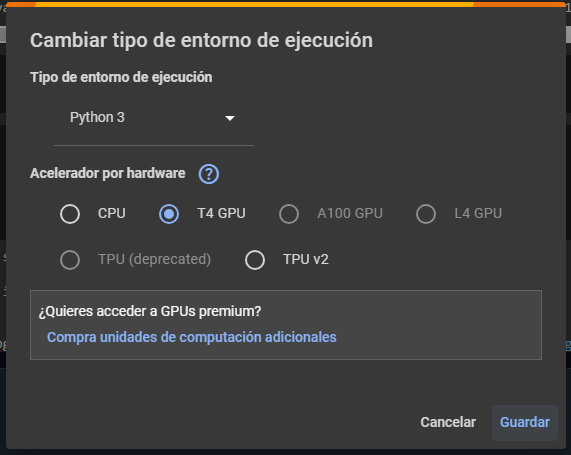
\includegraphics[width=1\textwidth]{img/aceleracion.png}
    \caption{Prestaciones LangChain, reuperado de \cite{retrieval}}
    \label{fig:acel}
\end{figure}

\subsection{Zube.io}

Zube.io es un gestor de proyectos que emplea metodologías ágiles como Kanban o Scrum. En este proyecto ha resultado útil para la planificación de tareas.

En el anexo A se puede encontrar un desglose detallado de cómo se ha empleado esta herramienta.

\subsection{Github}

GitHub es un gestor de repositorios en linea empleado fundamentalmente para la creación de código. Desde hace años resulta una herramienta indispensable para el desarrollo de software, permitiendo, entre otras cosas, la colaboración entre varios desarrolladores, el seguimiento del desarrollo mediante "issues" y la gestión de varios repositorios que pueden funcionar como portfolio o simplemente para almacenar código.

Todo el proyecto se encuentra público en el repositorio:\\
dlp1004/Aplicacion\_de\_chatbot\_con\_LLM\_y\_RAG\_para\_la\_gestion\_de\\\_informacion\_cientifica\_de\_COVID-19\_en\_PubMed

\subsection{Kaggle}

Kaggle es una comunidad centrada en la inteligencia artificial y el machine learning, tiene varias funcionalidades, entre ellas destaca la publicación de código, modelos y datasets, también se celebran en ella competiciones y discusiones sobre temas relacionados, para este proyecto su papel ha sido el de extraer los datos de entrenamiento, \cite{Anandhu_H_abstracts_2023}.

\subsection{Overleaf}

Overleaf es la herramienta en la que se está escribiendo toda esta documentación, se trata de un editor en linea de Latex, intuitivo y fácil de usar.

\subsection{ChatGPT}

Para tareas de traducción y redacción se ha empleado ChatGPT, otra herramienta de chatbot que emplea los LLMs GPT-3.5 y GPT-4, para más información sobre LLMs, dirigirse al capítulo 3 de esta memoria.

\subsection{Gradio}

Gradio es una librería diseñada para python que provee de un framework para realizar demos de interfaces para aplicaciones de machine learning, una ventaja de este paquete es que una interfaz de Gradio se puede integrar en notebooks de Python o presentarse como una página web.

Una interfaz de Gradio puede generar automáticamente un enlace público que puedes compartir con colegas, permitiéndoles interactuar con el modelo en tu computadora de forma remota desde sus propios dispositivos, lo que hace muy conveniente su utilización para una prueba de concepto.

Gradio también provee de servicios de Hosting permanente con su integración con los espacios de Hugging Face, lamentablemente este proyecto demanda una cantidad de gpu que escapa la disponible en el servicio de hosting gratuito.